\begin{frame}{}
    \LARGE Diffusion Models: \textbf{Reverse Denoising Process}
\end{frame}

\begin{frame}{Reverse Denoising Process}
    In the reverse denoising process, we denoise Gaussian noise to generate an image.
    \begin{itemize}
        \item<2-> We start with a sample from the noise distribution $p(\mathbf{x}_T) = \mathcal{N}(\mathbf{x}_T; 0, 1)$.
        \item<3-> The goal is to iteratively denoise this sample to recover the original image $\mathbf{x}_0$.
        \item<4-> At each time step $t$, we want to sample $\mathbf{x}_{t-1}$ given $\mathbf{x}_t$.
        \item<5-> The reverse process is defined as $p_\theta(\mathbf{x}_{t-1}|\mathbf{x}_t)$, which we will learn using a neural network.
    \end{itemize}
\end{frame}


\begin{frame}[allowframebreaks]{Reverse Denoising Process}
    \begin{itemize}
        \item The reverse process is a Markov chain that iteratively denoises the image.
        \item We want to sample $\mathbf{x}_{t-1}$ from $p_\theta(\mathbf{x}_{t-1}|\mathbf{x}_t)$.
        \item However, $p_\theta(\mathbf{x}_{t-1}|\mathbf{x}_t)$ is unknown and needs to be learned.
        
\framebreak
        
        \item We approximate it with a neural network that predicts the mean and variance of the Gaussian distribution.
        \item If $\beta_t$ is small enough at each time step, we can assume $p_\theta(\mathbf{x}_{t-1}|\mathbf{x}_t)$ is a Gaussian distribution:
        $$
        p_\theta (\mathbf{x}_{t-1} | \mathbf{x}_t) = \mathcal{N}(\mathbf{x}_{t-1}; \mu_\theta(\mathbf{x}_{t}, t), \Sigma_\theta (\mathbf{x}_{t}, t))
        $$
        where $\mu_\theta$ and $\Sigma_\theta$ are neural networks conditioned on $\mathbf{x}_t$ and $t$.
    \end{itemize}
\framebreak
    \begin{itemize}
        \item For simplicity, we can fix the variance $\Sigma_\theta$ to a constant value (e.g., $\beta_t \mathbf{I}$) and only learn the mean $\mu_\theta$.
        
\framebreak
        
        \item The reverse process can then be expressed as:
        $$
        p_\theta (\mathbf{x}_{t-1} | \mathbf{x}_t) = \mathcal{N}(\mathbf{x}_{t-1}; \mu_\theta(\mathbf{x}_{t}, t), \beta_t \mathbf{I})
        $$
        and the joint distribution over all time steps is:
        $$
        p_\theta(\mathbf{x}_{0:T}) = p(\mathbf{x}_T) \prod_{t=1}^T p_\theta (\mathbf{x}_{t-1} | \mathbf{x}_t)
        $$
    \end{itemize}
    \begin{figure}
        \centering
        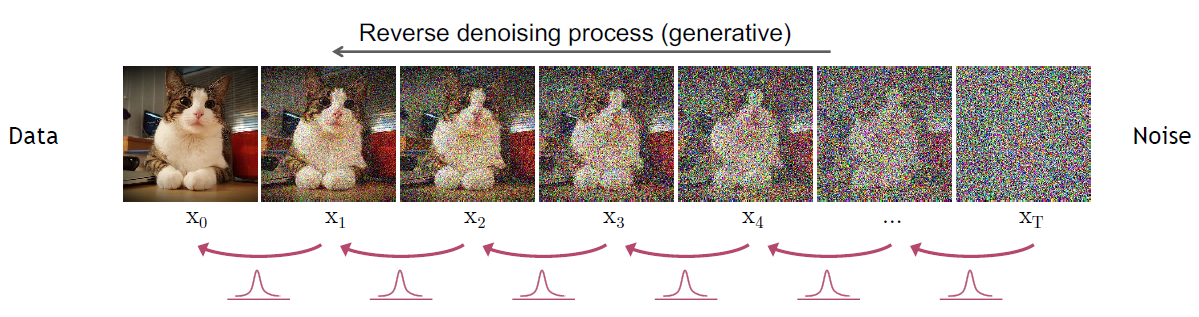
\includegraphics[height=0.4\textheight, width=\textwidth, keepaspectratio]{images/diffusion/diff_4.png}
        \caption*{Reverse denoising process in diffusion models.}
    \end{figure}
\end{frame}